\chapter{Broader Impact}
\label{chap:lipservice}

In this chapter I propose to add several enhancements to Landslide to apply its techniques beyond CMU's walls.
%with little to no manual instrumentation effort required.
This is the third of the three projects I am proposing for this thesis and so far exists only in dreams.
The project will have two parts: adding support for Pintos \cite{pintos}, and adding support for Transactional Memory \cite{transactional-memory}.

\section{Pintos}
\label{sec:pintos-todo}

The Pintos architecture \cite{pintos}, outlined in Section~\ref{sec:overview-pintos}, provides an opportunity to test Landslide's pedagogical mettle beyond CMU's walls.
However, the existing scheduler and concurrency primitives which Pintos provides somewhat limits the remaining concurrency-critical code left to write,
hence limiting the degree to which Landslide can test student submissions.
This is in contrast to the Pebbles assignments at CMU, in which students must implement all the functionality listed in Section~\ref{sec:overview-pintos}.
On the other hand, the upside of Pintos providing substantially more basecode than Pebbles is that most, if not all, of Landslide's kernel instrumentation can be done automatically,
using the names of the core scheduler functions already provided.
For the experiments in Chapter~\ref{chap:quicksand}, I already implemented rudimentary support to test Pintos kernels, but more remains to be done.

{\bf Stuff I already did.}
The existing Pintos support includes
a new set of annotations (e.g., {\tt mutex\_lock} in Pebbles is now called {\tt sema\_down};
handling several quirks of the basecode's scheduling behaviour (ask me if you really care to know);
extending the heap tracker to handle Pintos's page allocator {\tt palloc} as well as the kernel {\tt malloc},
as well as the fact that kernel memory is not direct-mapped like in Pebbles;
new thread-liveness code to detect when a test case terminates;
skipping some busy-wait loops in the boot sequence used for device communication,
a complicated fall-back case in Landslide's timer injection algorithm the workings of which I don't even remember anymore,
and extending the lock-set analysis to include Pintos's interrupt-disabling infrastructure (which was actually pretty tricky when using vector clocks for pure-HB).
All these features apply to behaviours included with the stock base-code, so should apply generally to all but the most adventurous student implementations.

{\bf Stuff I still need to do.}
However, as you might have guessed, there are still a few cases where the existing instrumentation is not fully general.
When preparing Chapter~\ref{chap:quicksand}'s experiments, I needed to adjust some student submissions to be compatible with Landslide's existing annotation process.
In order to distribute Landslide for student use beyond CMU, it will need to support these cases automatically.
These include:
\begin{itemize}
	\item Allowing for the priority scheduler's runqueues to be implemented as an array of queues, rather than the single queue head as provided in the basecode.
	\item Insert the {\tt tell\_landslide\_sleeping} annotation more intelligently than looking for a {\tt list\_insert\_ordered} call (a basecode function which most, but not all, students use).
	\item Some versions of the basecode distribute a {\tt sema\_up} implementation which {\tt yield}s unconditionally, which Landslide must bypass.
	\item Some students use {\tt timer\_sleep} or {\tt while (!flag) continue} when they should use {\tt yield}, which can lead to false-positive deadlocks if not automatically replaced.
	\item I'm sure I've forgotten some less-common ones, which I expect to handle on-the-fly when students email me Landslide crash reports.
\end{itemize}
When fixing my sample of Pintoses by hand, there were also myriad deterministic bugs, such as use-after-frees e.g.~arising from unsafe {\tt strlen} calls.
As with Pebbles student experiments, however, I intend the students to encounter such bug reports and fix them on their own, despite not being concurrency bugs.
It would be a Ph.D. unto itself to automatically ensure stable determinized execution of arbitrary student code.
Actually, probably outright impossible.

{\bf New emulation platform.}
Most importantly, I will need to free Landslide from its dependence on Simics, which requires paid licenses for use beyond CMU's walls.
Other candidate emulation (simulation or virtualization) platforms for Landslide include Bochs, QEMU, VMWare, and Xen.
I am presently studying which of these will most suit Landslide's needs,
but so far Bochs seems like the best bet, which happens to be the simulator used at Berkeley, Stanford, and U. of Chicago anyway.

{\bf Experimental goals.}
Having only one semester (ideally; or two, if my timeline ends up delayed) to test Landslide with Pintos students,
I'll be unable to gather as comprehensive a dataset as I have with 15-410 at CMU.
This will serve more as a proof-of-concept, demonstrating that MC can realistically replace stress testing in operating systems courses worldwide.
Nevertheless, I intend also to analyze what little data I can gather, comparing the incidences and types of bugs found between Pebbles and Pintos populations.
This will perhaps shed light on the advantages and/or shortcomings of either project,
leading to recommendations for improving either project's educational value (independently of using MC).

\section{Transactional Memory}
\label{sec:tm}

Transactional Memory (TM) is a mechanism by which programmers may avoid conventional concurrency primitives, optimizing for performance in the common case when threads do not conflict.
A transactional program surrounds its critical section(s) with transaction begin/end statements, which ensure that no other thread can observe an intermediate state during the transaction.
If a conflict is observed, the transaction {\em aborts}, rolling the program back to the transaction's initial state, and executing an optional back-up code path.
The programmer may also explicitly abort the transaction using an abort statement.
An example transactional program is shown in Figure~\ref{fig:txn-example}.

\begin{figure}[t]
	\begin{center}
	\begin{tabular}{ll}
		\multicolumn{2}{c}{Initially {\tt int foo, bar = 0; mutex\_t m;}} \\
		\\
		\begin{tabular}{l}
		{\bf Thread 1} \\
		\hline
		\texttt{if (\_xbegin() ==} \\
		\texttt{~~~~~~~~\_XBEGIN\_STARTED) \{} \\
		\texttt{~~~~foo++;} \\
		\texttt{~~~~\_xend();} \\
		\texttt{\} else \{} \\
		\texttt{~~~~mutex\_lock(\&m);} \\
		\texttt{~~~~assert(foo > 0 ||} \\
		\texttt{~~~~~~~~~~~bar > 0);} \\
		\texttt{~~~~mutex\_unlock(\&m);} \\
		\texttt{\}} \\
		\end{tabular}
		&
		\begin{tabular}{l}
		{\bf Thread 2} \\
		\hline
		\texttt{if (\_xbegin() ==} \\
		\texttt{~~~~~~~~\_XBEGIN\_STARTED) \{} \\
		\texttt{~~~~bar++;} \\
		\texttt{~~~~\_xend();} \\
		\texttt{\} else \{} \\
		\texttt{~~~~mutex\_lock(\&m);} \\
		\texttt{~~~~assert(foo > 0 ||} \\
		\texttt{~~~~~~~~~~~bar > 0);} \\
		\texttt{~~~~mutex\_unlock(\&m);} \\
		\texttt{\}} \\
		\end{tabular}
	\end{tabular}
	\end{center}
	\caption{Example transactional program, written using GCC's transactional memory compiler intrinsics \cite{htm-gcc}.
	%The x86 assembly instructions are named {\tt xbegin}, {\tt xend}, and {\tt xabort}; I have named the functions of this imaginary C interface the same.
	Different behaviours are possible depending whether the transactions are backed by HTM or STM.}
	\label{fig:txn-example}
\end{figure}

TM may be implemented either in hardware (HTM) \cite{htm-haswell}, or in software (STM) \cite{stm-pldi06}.
Though their interfaces to the programmer are similar, their semantics demand a slightly different treatment from Landslide's perspective.
The key difference is that HTM transactions may fail for any reason, beyond the scope of the program's behaviour, such as the CPU's cache being too full.
STM transactions, on the other hand, will fail only if an actual conflict is observed from another thread.

Consider again the example program: The transactions of the two threads do not conflict, so they may abort only under HTM.
However, when they abort for a reason other than a conflict on {\tt foo} or {\tt bar}, the assertions in the backup code will fail.
Hence, some programs which are correct under STM may contain bugs under HTM.
Supporting TM in Landslide will consist of several steps, extending the concurrency model to incorporate failure injections and extending DPOR to determine when transaction aborts are possible depending on the underlying TM mechanism.

\subsection{HTM}

{\bf Mutex isomorphism.}
When modelling TM in Landslide, we do not care about fidelity to performance characteristics or non-observable roll-back semantics.
The goal of model checking is to exercise all observable program behaviours,
so Landslide can model the execution of transactional programs using existing primitives if possible.
In the first stage of the project, I will prove that a transactional program using is equivalent to one with a global mutex swapped for its {\tt xbegin}s and {\tt xend}s (assuming a retry-only policy for handling aborts).
This will allow Landslide to test all observable TM behaviours using its existing infrastructure for mutexes,
rather than relying on the platform providing accurate TM emulation.

{\bf Abort nondeterminism.}
Next, I will extend the concurrency model to support the nondeterminism arising from transaction aborts.
During execution, Landslide inject a failure to force threads to branch into backup code paths.
Failure injections add an extra ``dimension'' of non-determinism:
at each {\tt xbegin} operation which is a preemption point, Landslide may force a normal context switch to re-interleave threads, or it may inject a transaction abort to test the backup code.
(This also avoids the need to speculatively execute and/or roll-back failing transactions.)
Because HTM transactions can fail for any reason, outside of the programmer's control, Landslide's DPOR implementation will consider failure injections always ``enabled''.

{\bf Reduction challenge.}
I've identified a case under abort nondeterminism in which the current implementation of DPOR will fail to achieve a possible reduction.
Let $1A$, $1B$, $2A$, and $2B$ denote the transitions which execute the {\tt if} and {\tt else} branches by each thread, respectively.
Note that $1A$ conflicts with $2B$, and $1B$ with $2A$, but $1A$ and $2A$ are independent, as are $1B$ and $2B$.
Figure~\ref{fig:txn-graph} provides a visual aid.
There are two possible reductions: pruning $2A,1A$ after testing $1A,2A$, and pruning $2B,1B$ after testing $1B,2B$;
in other words, branches 5 and 8 can be skipped.
However, %if we simply extended DPOR to always inject failures when possible,
our current DPOR implementation will tag the $2B$ subtree to explore after observing the conflict in branch 2 (likewise the $2A$ subtree from branch 3),
but then have no memory of whether it was subsequently supposed to run $1A$ or $1B$, and have to try both.
To fix this will require an optimization analogous to ``sleep sets'' \cite{dpor}:
the tag to explore the $2A$ or $2B$ subtree must include an annotation to remember whether or not the conflict arose after a failure injection in $1$.

\begin{figure}[t]
	\begin{center}
		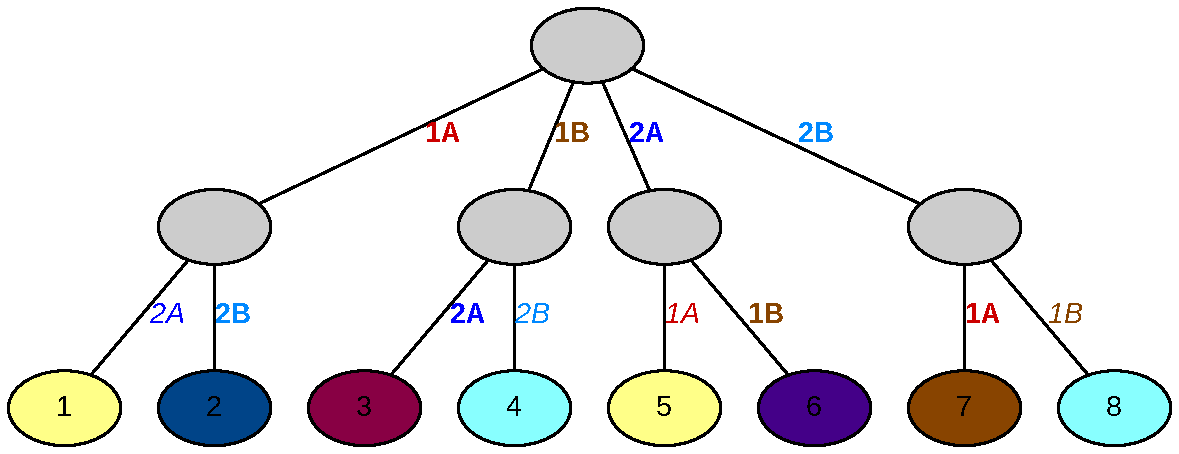
\includegraphics[width=0.8\textwidth]{htm-graph.pdf}
	\end{center}
	\caption{State space corresponding to the program in Figure~\ref{fig:txn-example}.
	Conflicting transitions are marked in bold;
	transitions which are independent from their predecessors are italicized.
	End states colored the same (the cyan and yellow ones) are equivalent.
	}
	\label{fig:txn-graph}
\end{figure}

\subsection{STM}

STM transactions abort only when multiple threads conflict.
Because Landslide already computes memory conflicts among each pair of transitions, it will be natural to extend DPOR to consult the conflict set when deciding whether to exercise a failure injection.
I will extend Landslide in this manner, and even support programs with both types of transactions, as long as the different {\tt xbegin} invocations are suitably annotated.

\subsection{Hybrid HTM/STM}

A recent paper \cite{hybrid-htm-stm} introduced several ways of combining HTM and STM in the same program, nesting transactions of different types.
It presented several semantics for such transactions transactions, the most interesting of which being ``open nesting'', in which a nested transaction's state becomes visible to other threads even during a containing transaction.
That state can then be rolled back if the latter aborts.
I plan to develop a theoretical model for how such transactions would affect Landslide's concurrency model,
although I expect to relegate any implementation thereof to future work.
